\chapter{Ansatz für eine skalierbare und flexible Softwareentwicklungsumgebung}
\label{ch:chapter04}

\section{Veränderung der Rahmenbedingungen}

Die Entwicklung eines flexiblen und skalierbaren Systems und Umgebung für die Softwareentwicklung innerhalb von Banken erfordert wesentliche Veränderungen in den Strukturen der IT-Bereiche der Institute und in ihrem Ablauf. Wesentlicher Faktor ist hierfür die Tatsache, dass die Anwendungen und Systeme für die Softwareentwicklung ständigen Veränderungen ausgesetzt sind. Standards in der Softwareentwicklung sind mittlerweile agil und verändern sich kontinuierlich und dynamisch. Eine flexible IT-Architektur ist erforderlich, um sich diesen Veränderungen anzupassen.
\medskip
\\
Bussmann et al. nennt zwei Wege für den Ersatz und grundlegenden Re-Design von Kernsystemen: \cite{Bussmann2006}
\begin{itemize}
    \item Anwendungen schrittweise entkernen, erneuern und modularisieren und funktionale Anforderungen konsolidieren
    \item Kernsysteme durch völlig neue, selbst entwickelte Applikationen austauschen oder einsetzen von Standardsoftware
\end{itemize}
%

Die unflexible IT-Architektur in Banken ist keine neue Erkenntnis und wird schon lange in der entsprechenden Literatur gefordert. Mittlerweile darf nicht mehr von Bedarf oder Forderung gesprochen werden. Veränderungen werden nicht nur durch ein Wertschöpfungspotenzial hervorgerufen. Viel mehr wird die IT in Betrieben mit alten Strukturen durch äußere Kräfte gezwungen sich anzupassen. Grundlage hierfür sind neue Technologietrends \cite{Bussmann2006}, die mittlerweile in ihrer Auswirkung jedoch gravierender sind. Eine entsprechende Verdrängung im Wettbewerb kann viel schneller erfolgen als bisher. Neben Impulse für Innovation kann eine Disruption durch neue Technologietrends beobachtet werden.
\medskip
\\
Verdrängungen finden nicht nur durch eine Konkurrenz auf gleicher Augenhöhe statt. Eine Verdrängung kann auch unerwartet von kleinen Betrieben mit effizienten Abläufen kommen, die durch Schnelligkeit, Verfügbarkeit, Skalierbarkeit und Qualität ihrer Leistungen überzeugen kann.  Gerade im Bankwesen könnten Verdrängungen stattfinden, die jenseits der bisherigen Rahmenbedingungen agieren. Der hierfürige Technologietrend könnte beispielsweise die Blockchain-Technologie sein. Analog zum genossenschaftlichen Prinzip der Selbsthilfe, Selbstverantwortung und Selbstverwaltung könnten unabhängige Organisationen entstehen, nach dem historischen Muster, aus denen die Genossenschaften stammen. 

\paragraph{IT als Kernkompetenz} Bussmann et al. bezeichnet die IT als Kernkompetenz. IT-Anwendungen unterscheiden sich in zwei Bereiche, in welcher Technologietrends zu innovativen Lösungen führen. Neben den Anwendungen für den Dialog mit Kunden sind es Anwendungen zur Steuerung und Unterstützung von internen Prozessen, die gerade im Finanzwesen mit steigenden Anforderungen nicht mithalten können. \cite{Bussmann2006}
\medskip
\\



\paragraph{Plattform durch IT}
Ausschlaggebend ist hierfür die Bereitstellung einer Plattform, auf welcher eine ganze Wertschöpfungskette entsteht.

\paragraph{Relevanz der BaFin Anforderungen für Entwickler}
Die BaFin Anforderungen, Gängige Sicherheitsstandards und weitere Vorschriften sind für Entwickler wichtig, um ihre Verantwortung über die IT-Risiken in Banken und anderen systemrelevanten Betrieben zu verstehen. Insbesondere sind sie für die Entwicklung nachvollziehbarer Systeme für ihren nachhaltigen Betrieb, Überwachung und Überprüfung zu berücksichtigen. Um verwachsene und unflexible Architekturen zu vermeiden sollten Entwickler, im Bereich der Anwendungen, die interne Prozesse unterstützen \cite{Bussmann2006}, sich mit diesem Thema auseinandersetzen.

Neben den Leistungsansprüchen sollten die Sicherheitsansprüche im Vordergrund stehen. Die Implementierung von neuen Technologien wirft bei wesentlichen Veränderungen viele Compliancefragen auf \cite{MaRisk:2017}. Diese hängen mit den Sicherheitsansprüchen zusammen. 

\paragraph{Idee für ein innovatives Risikomanagement}
Die von Disterer beschriebenen Probleme im Betrieb von Anwendungen durch die mangelnde Beachtung von nichtfunktionalen Anforderungen und die Einführung von Quality Gates \cite{mci/Disterer2011} kann hierbei auf Probleme für die internen Kontrollverfahren ausgeweitet werden. Eine Koordination zwischen Entwicklung und Betrieb sollte das IT-Risikomanagement miteinbeziehen. Dabei darf die Geschwindigkeit des Entwicklungs- oder Integrationsprozesses nicht beeinträchtigt werden. Die Schnelligkeit hat bei der Beantwortung von Compliancefragen eine wichtige Rolle. Entwickler könnten zuerst die Prozesse des IT-Risikomanagements optimieren und automatisieren, um sich Handlungsfreiheit für Innovation und wesentlichen Veränderungen innerhalb der Organisation zu schaffen. Sie sollten in das Risikomanagement integriert werden. Ein Entwickler aus einem anderen Projekt könnte als Compliance- und Risikoverantwortlicher parallel wichtige Compliancefragen auf technischer Ebene schnell überprüfen und vorab beantworten. Dadurch könnte unter Vorbehalt schon mit neuen Technologien und Methoden an Lösungen gearbeitet werden oder Veränderungen in Gang gesetzt werden. Um einer Disruption zu begegnen ist das Risiko von verschwendetem Aufwand in Kauf zu nehmen, um sich eine Anpassungs- und Reaktionsfähigkeit zu schaffen, die geschäftskritisch ist.


\section{Nachvollziehbarkeit der SEU}



\paragraph{Repository für Artefakte}
Hierfür wird ein Repository zum Speichern der Artefakte angewendet. Eine Standardsoftware für ein Artefaktrepository ist die Anwendung Artifactory. Dieser speichert mit einem Snapshot die Ergebnisse aus dem Build-Job. Das Artifactory wird ebenfalls verwendet, um die Ressourcen sowie Libraries für den Build zu beziehen. Artifactory wird hierbei entweder als Proxy für den Zugriff auf ausgesuchte öffentliche Repositories verwendet oder die Ressourcen werden in der Artifactory Instanz gehostet.

\section{Skalierung von Jenkins mit Kubernetes}
Üblicherweise werden Anwendungen mit Kubernetes mit Replikas skaliert. Das heißt in der Praxis, dass eine neue Instanz der Anwendung erzeugt wird. Das bedeutet eine horizontale Skalierung von Anwendungen. Jenkins besteht bei einer Konfiguration mit verteilten Builds aus mehreren Komponenten. Ein Jenkins Master, dass die Build-Jobs triggert und ausführende Komponenten, die aus mehreren Agenten bestehen. Daher sollten die Komponenten für die Skalierung getrennt berücksichtigt werden. Die Skalierung ist vorwiegend für die ausführenden Komponenten erforderlich. 
\medskip
\\
Google beschreibt einen Ansatz für eine skalierbare Architektur von Jenkins mit der \ac{GKE}:

\begin{figure}[htbp]
 \centering
 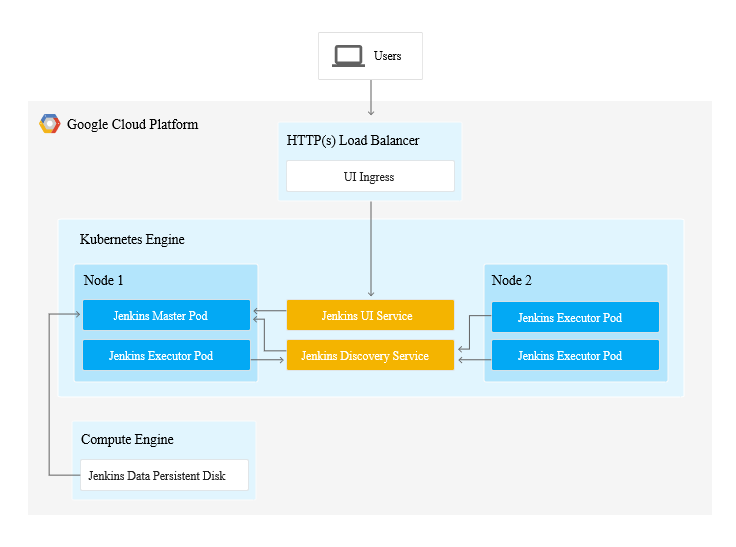
\includegraphics[width=1.0\textwidth]{gfx/jenkins-kubernetes-architecture.png}
 \caption{Deployment von Jenkins in einem Kubernetes Cluster mit mehreren Knoten \cite{Google:GKEJenkins}}
\end{figure}
Hierin werden die Komponenten in einem Node zusammengefasst. In Node 1 befindet sich der Jenkins Master. Innerhalb dieses Nodes kann der Jenkins Master repliziert werden. Im gleichen Node oder in weiteren Nodes können die Jenkins Agenten, genannt Jenkins Executor, erzeugt werden.


\subsection{Anlegen eines Kubernetes Clusters für Jenkins}
Pathania beschreibt in \cite{Pathania2017}, wie Jenkins mit \ac{GCP} und Kubernetes und Docker skaliert werden kann. Hierbei geht er genau auf die Konfiguration von Kubernetes und der \ac{GCP} ein.


\paragraph{Google Kubernetes Engine}

\paragraph{Minikube}



\paragraph{Jenkins Master-Agent Konfiguration}


\paragraph{Sonstige Konfigurationen}

\subsection{Jenkins Agents}

\paragraph{Virtuelle Maschinen}

\paragraph{Docker}

\paragraph{Minimale Images}

\subsection{Layering}

\section{Entwicklung von Docker-Images für Jenkins Agenten}

Während des Entwurfs der Architektur eines ganzen Systems für die Softwareentwicklung gibt es viele Parameter, die sich ständig Verändern können. Beispielsweise kann die Entscheidung für oder gegen eine Public-Cloud offen stehen oder es stehen Anpassungen offen, die entscheidende Auswirkungen auf die Teilsysteme haben.
Für einen kleinsten gemeinsamen Nenner in der Entwicklung eines Systems sollte die Anwendung modularisiert werden und anhand ihrer wesentlichen Funktion kann anschließend die Entwicklung parallel durchgeführt werden. Grundlage hierfür bieten die Microservice Architekturen. Für die Build-Jobs ist die Lokalität erstmal nicht wichtig. Für sie ist die Ausstattung mit den nötigen Build-Tools wichtig und die Kommunikation mit der Versionsverwaltung, gleichzeitig auch die Kommunikation zum integrierenden System. Daher kann bereits mit der Entwicklung von Images für Container begonnen werden, während wichtige Aspekte des Gesamtsystems noch offen stehen.

\paragraph{Use-Case}
Die Images werden zur Erzeugung von Containern innerhalb eines Kubernetes Clusters für die Integrationsplattform Jenkins verwendet. Diese werden erzeugt, für den Einsatz als Agent innerhalb einer Master-Slave Konfiguration von Jenkins für verteilte Builds. Diese Agenten sind für die Ausführung eines Java Builds mit dem Build-Management Tool Maven zuständig.

\paragraph{Anforderungen}
\begin{itemize}
    \item Aufgrund von hohen Gebühren für cloud-out-traffic soll die Image möglichst klein sein
    \item Die Umgebung soll \ac{JDK11} und Maven enthalten und entsprechend konfiguriert werden
    \item Beim Bauen der Image sollen alle Ressourcen intern über eine private Artifactory-Instanz bezogen werden
    \item Zum Erstellen eines Builds soll Maven mit Artifactory kommunizieren und Daten übertragen können
    \item Zur Evaluation der Umgebung soll Maven einen erfolgreichen Build zu einem Testprojekt erstellen
\end{itemize}



\subsection{Auswahl eines Basis-Image}
Der erste Schritt in einem Dockerfile ist das Festlegen eines Basis-Images, aus welcher die Umgebung konfiguriert werden soll. Hierzu wird am Anfang der Dockerfile \lstinline{FROM image:tag} definiert. Theoretisch kann eine Image auch aus einer leeren Umgebung \lstinline{FROM scratch} erzeugt werden. Das ist jedoch unüblich, selbst bei Containern für embedded Systeme.

Hierzu gibt es im Docker-Hub öffentliche Images, die umkonfiguriert werden können. Die offizielle Maven image \lstinline{maven:3.6.3-jdk-11}, die Maven und JDK11 bereits installiert hat, könnte beispielsweise für eine einfache Anwendung verwendet werden. Für den Use-Case innerhalb der Continuous Integration Plattform können die potenziellen Basis-Images aus dem Dockerhub zwischen folgenden Stufen in ihrer Ausstattung unterschieden werden:
\begin{enumerate}
    \item Betriebssystem: \lstinline{ubuntu, debian, alpine}
    \item SDK: \lstinline{jdk11, openjdk11, adoptopenjdk11, amazoncoretto11}
    \item Build-Management: \lstinline{maven}
\end{enumerate}
Bei einer hohen Ausstattungsstufe besteht jedoch eine hohe Abhängigkeit von einer bestimmten Image, die wiederrum auf niedrigeren Stufen basiert. Für eine möglichst hohe Nachvollziehbarkeit wäre es sinnvoll eine möglichst niedrige Stufe zu wählen und die Umgebung innerhalb der eigenen Infrastruktur zu konfigurieren. Für eine möglichst hohe Effizienz der Container sind jedoch umfangreiche Kenntnisse über Betriebssysteme erforderlich. Diese fällt je nach Umfang in den Tätigkeitsbereich eines Systementwicklers.

\paragraph{Vorteile von selbst gebauten Images}
Für das Gesamtbild der Skalierbarkeit ist es jedoch sinnvoll das Ganze mit einer hohen Kompetenz anzugehen. Möglichst minimale und effiziente Container-Umgebungen wirken sich kumulativ auf den Ressourcenbedarf des ganzen Clusters aus. Bei einer Public-Cloud werden üblicherweise die genutzten Ressourcen mit einem Studensatz abgerechnet. Ein weiterer Vorteil entsteht durch das Prinzip des Layerings bei Container-Umgebungen. Auf einer eigenen Image können weitere Images basieren. Hierdurch muss lediglich eine Basis-Image entwickelt werden, in welchem nur die essentiellen Anpassungen vorgenommen werden, mit dem Ziel ein intern evaluiertes Betriebssystem bereitzustellen. Basierend hierauf können unabhängig voneinander Images aufbauen mit den entsprechenden Tools für die unterschiedlichen Programmiersprachen. Dadurch entsteht eine hohe Synergie und Flexibilität für die Systementwicklung und den Betrieb der Systeme.

\paragraph{Minimale Images}
Eine Best-Practice innerhalb der Entwicklung von Docker-Images ist ihre Größe so niedrig wie möglich zu halten. 

Die Linux-Image \lstinline{alpine} ist hierfür als Basis-Image besonders beliebt, da sie mit einer Größe von nur \lstinline{5 MB} eine Linux-Umgebung abbildet und eine Package-Repository besitzt \cite{docker-alpine}. Alpine benutzt jedoch nicht die C Standardlibrary \lstinline{glibc}, sondern \lstinline{musl libc} \cite{alpine-about}. Daher sollte die Nutzung gerade zum Kompilieren von Quellcode abgewägt werden.
Auch mit den offiziellen Docker-Images von Ubuntu und Debian kommt man auch mit entsprechenden Praktiken auf eine niedrige Größe. Für den Anwendungsfall innerhalb der \ac{CI} Plattform ist es wichtig eine kleinstmögliche Java Installation durchzuführen. Hierfür gibt es entsprechende \lstinline{slim} Editionen der JDK. 

Ein Vergleich zwischen der normalen \lstinline{openjdk:11-jdk} mit der \lstinline{-slim}\footnote{Vgl. Images aus index.docker.io}:
\begin{verbatim}
openjdk:11-jdk
SIZE 306.67 MB
sha256:9efbdac6886418e7c473ee4d59ff728d029fad773364cb671794333d-
d16e4158

openjdk:11-jdk-slim
SIZE 216.36 MB
sha256:a67455311b2982c4cb795c8a38d55cf17e840c8fdb9ca82d14cd38d8-
43e24111
\end{verbatim}

Beide Images basieren auf \lstinline{debian:buster}, wobei die zweite Image auf \lstinline{debian:buster-slim} basiert.

Ein vergleich zwischen \lstinline{alpine:3.12} und \lstinline{debian:buster-slim}
\begin{verbatim}
alpine:3.12
SIZE 2.3 MB
sha256:c929c5ca1d3f793bfdd2c6d6d9210e2530f1184c0f488f514f1bb808-
0bb1e82b

debian:buster-slim
SIZE 26.46 MB
sha256:9f8288b62780eaa2ee6341c6f8632990eae83d9b1caac9d0e4545e6f-
c8ce5e6d
\end{verbatim}

Auf die absolute Größe kommt es nicht an. Viel wichtiger ist es bei der Konfiguration der Images sich genau mit den Layers zu befassen. Jedes Befehl in der Dockerfile erzeugt einen neuen Layer. Das Löschen von Dateien wirkt sich nicht auf die vorigen Layer aus. Daher sollten Befehle verkettet als ein Befehl ausgeführt werden und möglichst wenige Daten erzeugt werden. 
\medskip
\\
Aufgrund der geringen Auswirkung der absoluten Größe wird möglichst auf eine Standardumgebung als Basis-Image verwendet. Hierfür wurde \lstinline{debian:buster-slim} ausgewählt. Die Debian Image auf Dockerhub ist eine offizielle Image, die hauptsächtlich vom Debian Maintainer tianon gepflegt und veröffentlicht wird \cite{docker-debian-builds, docker-debian}.

\subsection{Konfiguration der Images}

\paragraph{Kommunikation mit Artifactory}

\paragraph{Bezug von Build-Tools über Artifactory}

\paragraph{Installation von Java}

\paragraph{Cacerts}

\paragraph{Installation von Maven}

\paragraph{Konfiguration von Maven}

\paragraph{Einfügen eines Testjobs}

\subsection{Bauen von Images}

\subsection{Evaluation der Images}

\subsection{Bereitstellung der Images}

\subsection{Integration in Jenkins}

\paragraph{SSH}

\paragraph{JNLP}